

\documentclass[pfe]{./configs/isipfe}
% \documentclass[]{./configs/isipfe}
% \graphicspath{{./img/}}
\usepackage{listings}
\usepackage{xcolor}
\usepackage{indentfirst}

\setstretch{1.1}

\definecolor{codegreen}{rgb}{0,0.6,0}
\definecolor{codegray}{rgb}{0.5,0.5,0.5}
\definecolor{codepurple}{rgb}{0.58,0,0.82}
\definecolor{backcolour}{rgb}{0.95,0.95,0.92}

\lstdefinestyle{mystyle}{
    backgroundcolor=\color{backcolour},   
    commentstyle=\color{codegreen},
    keywordstyle=\color{codegreen},
    numberstyle=\tiny\color{codegray},
    stringstyle=\color{codepurple},
    basicstyle=\ttfamily\footnotesize,
    breakatwhitespace=false,         
    breaklines=true,                 
    captionpos=b,                    
    keepspaces=true,                 
    numbers=left,                    
    numbersep=5pt,                  
    showspaces=false,                
    showstringspaces=false,
    showtabs=false,                  
    tabsize=2
}

\lstset{style=mystyle }


%=========== File containing some new commands ============%
%                                                          %
% Copyright (C) ISI - All Rights Reserved                  %
% Proprietary                                              %
% Written by Med Hossam <med.hossam@gmail.com>, April 2016 %
%                                                          %
% @author: HEDHILI Med Houssemeddine                       %
% @linkedin: http://tn.linkedin.com/in/medhossam           %
%==========================================================%

\newenvironment{changemargin}[2]{%
\begin{list}{}{%
\setlength{\leftmargin}{#1}%
\setlength{\rightmargin}{#2}%
}%
\item[]}
{\end{list}}

\makeatletter

%================= front cover variables =================%
%\renewcommand{\contentsname}{Table of Contents}
%\renewcommand{ \tableofcontents}{Table of Contents}

\newcommand{\secondAuthor}[1]{\gdef\@secondAuthor{#1}}%
\newcommand{\@secondAuthor}{\@latex@warning@no@line{No \noexpand\secondAuthor given}}

\newcommand{\diplomaName}[1]{\gdef\@diplomaName{#1}}%
\newcommand{\@diplomaName}{\@latex@warning@no@line{No \noexpand\diplomaName given}}

\newcommand{\speciality}[1]{\gdef\@speciality{#1}}%
\newcommand{\@speciality}{\@latex@warning@no@line{No \noexpand\speciality given}}

\newcommand{\proFramerName}[1]{\gdef\@proFramerName{#1}}%
\newcommand{\@proFramerName}{\@latex@warning@no@line{No \noexpand\proFramerName given}}

\newcommand{\proFramerSpeciality}[1]{\gdef\@proFramerSpeciality{#1}}%
\newcommand{\@proFramerSpeciality}{\@latex@warning@no@line{No \noexpand\proFramerSpeciality given}}

\newcommand{\academicFramerName}[1]{\gdef\@academicFramerName{#1}}%
\newcommand{\@academicFramerName}{\@latex@warning@no@line{No \noexpand\academicFramerName given}}

\newcommand{\academicFramerSpeciality}[1]{\gdef\@academicFramerSpeciality{#1}}%
\newcommand{\@academicFramerSpeciality}{\@latex@warning@no@line{No \noexpand\academicFramerSpeciality given}}

\newcommand{\collegeYear}[1]{\gdef\@collegeYear{#1}}%
\newcommand{\@collegeYear}{\@latex@warning@no@line{No \noexpand\collegeYear given}}

\newcommand{\companyName}[1]{\gdef\@companyName{#1}}%
\newcommand{\@companyName}{\@latex@warning@no@line{No \noexpand\companyName given}}

%================== Signatures variables ==================%

\newcommand{\proSignSentence}[1]{\gdef\@proSignSentence{#1}}%
\newcommand{\@proSignSentence}{\@latex@warning@no@line{No \noexpand\proSignSentence given}}

\newcommand{\academicSignSentence}[1]{\gdef\@academicSignSentence{#1}}%
\newcommand{\@academicSignSentence}{\@latex@warning@no@line{No \noexpand\academicSignSentence given}}

%================== Backcover variables ==================%

\newcommand{\arabicAbstract}[1]{\gdef\@arabicAbstract{#1}}%
\newcommand{\@arabicAbstract}{\@latex@warning@no@line{No \noexpand\arabicAbstract given}}

\newcommand{\arabicAbstractKeywords}[1]{\gdef\@arabicAbstractKeywords{#1}}%
\newcommand{\@arabicAbstractKeywords}{\@latex@warning@no@line{No \noexpand\arabicAbstractKeywords given}}

\newcommand{\frenchAbstract}[1]{\gdef\@frenchAbstract{#1}}%
\newcommand{\@frenchAbstract}{\@latex@warning@no@line{No \noexpand\frenchAbstract given}}

\newcommand{\frenchAbstractKeywords}[1]{\gdef\@frenchAbstractKeywords{#1}}%
\newcommand{\@frenchAbstractKeywords}{\@latex@warning@no@line{No \noexpand\frenchAbstractKeywords given}}

\newcommand{\englishAbstract}[1]{\gdef\@englishAbstract{#1}}%
\newcommand{\@englishAbstract}{\@latex@warning@no@line{No \noexpand\englishAbstract given}}

\newcommand{\englishAbstractKeywords}[1]{\gdef\@englishAbstractKeywords{#1}}%
\newcommand{\@englishAbstractKeywords}{\@latex@warning@no@line{No \noexpand\englishAbstractKeywords given}}

\newcommand{\companyEmail}[1]{\gdef\@companyEmail{#1}}%
\newcommand{\@companyEmail}{\@latex@warning@no@line{No \noexpand\companyEmail given}}

\newcommand{\companyTel}[1]{\gdef\@companyTel{#1}}%
\newcommand{\@companyTel}{\@latex@warning@no@line{No \noexpand\companyTel given}}

\newcommand{\companyFax}[1]{\gdef\@companyFax{#1}}%
\newcommand{\@companyFax}{\@latex@warning@no@line{No \noexpand\companyFax given}}

\newcommand{\companyAddressFR}[1]{\gdef\@companyAddressFR{#1}}%
\newcommand{\@companyAddressFR}{\@latex@warning@no@line{No \noexpand\companyAddressFR given}}

\newcommand{\companyAddressAR}[1]{\gdef\@companyAddressAR{#1}}%
\newcommand{\@companyAddressAR}{\@latex@warning@no@line{No \noexpand\companyAddressAR given}}

%============= cmd for inserting blank page =============%
\newcommand\blankpage{%
    \null
    \thispagestyle{empty}%
    \addtocounter{page}{-1}%
    \newpage}

%================ document main language ================%
\selectlanguage{English}
%\selectlanguage{english}

%================== required packages ===================%

\usepackage{tcolorbox}
\usepackage{afterpage}
\usepackage{array,longtable,multirow}% http://ctan.org/pkg/{array,longtable,multirow}
\usepackage{pifont}

\usepackage{pdflscape}
\usepackage{rotating}
\usepackage{wrapfig}

\usepackage[french]{babel}
\usepackage[utf8]{inputenc}

\usepackage{titlesec}

% Define a command to add indentation after section and subsection titles
\newcommand{\sectionindent}{\hspace{\parindent}}

% Customize section and subsection formatting
\titleformat{\section}{\normalfont\Large\bfseries}{\thesection}{1em}{}
\titleformat{\subsection}{\normalfont\large\bfseries}{\thesubsection}{1em}{}

% Add indentation after section and subsection titles
\titlespacing*{\section}{20pt}{3.5ex plus 1ex minus .2ex}{1.5ex plus .2ex}
\titlespacing*{\subsection}{20pt}{3.25ex plus 1ex minus .2ex}{1.5ex plus .2ex}

\makeindex

\begin{document}
    
\newcolumntype{L}{>{\raggedright\arraybackslash}}
\newcolumntype{R}{>{\raggedleft\arraybackslash}}
\newcolumntype{C}{>{\centering\arraybackslash}}
%==================================================%

%========= Config the cover section ==========%

\title{Développement d'une plateforme E-learning}

\author{Asma Ben Ayech}
%%% if necessary
% Set isBinomal to true and type second author name
%\setboolean{isBinomal}{true}
%\secondAuthor{Prénom NOM}

\diplomaName{Licence en ingénieurie des systémes informatiques}
\speciality{IOT}

%% Encadrant professionnel
\proFramerName{Ouertani Abderahim}


%% Encadrant académique
\academicFramerName{Amdouni Asma}


%% Entreprise d'accueil
\companyName{Inno-Think}

%% Année universitaire
\collegeYear{2023 - 2024}

%%%%%% Signatures section %%%%%%

% You can simply remove theses sentences by typing an empty string
% \proSignSentence{}

\proSignSentence{J'autorise l'étudiant à faire de son rapport de stage en vue d'une soutenance.}

\academicSignSentence{J'autorise l'étudiant à faire de son rapport de stage en vue d'une soutenance.}

%%% AR
\arabicAbstract{تم إنجاز هذا العمل داخل شركة اكتيا من أجل التحقق من صحة التدريب الإلزامي للحصول على الدبلوم الوطني للترخيص في العلوم التطبيقية والتكنولوجيا.
يتكون المشروع من تصميم تطبيق ويب باستخدام Visual Studio Code كبيئة تطوير.
الهدف من منصتي هو اكتشاف جميع أنواع البيانات المسربة في الويب المظلم والإبلاغ عن النتائج.}



%% To use latin characters inside the arabic text
% just put them inside the command \textLR{}
%%%%

%%% FR
\frenchAbstract{Ce travail a été réalisé au sein de l'entreprise ACTIA ES afin de valider le stage obligatoire pour l'obtention du Diplôme National de Licence en Sciences Appliquées et Technologie.
Le projet consiste à concevoir une application web utilisant Visual Studio Code comme environnement de développement.
L'objectif de ma plateforme est de détecter toutes sortes de fuites de données dans le Dark Web et de rapporter les résultats.}


%%% EN
\englishAbstract{This work was realized within the company ACTIA ES in order to validate the compulsory internship for the obtaining of the National Diploma of License in Applied Sciences and Technology. 
The project consists of designing a web application using Visual Studio Code as development environment. 
The objective of my platform is to Detect all kinds of leaked data in the Dark Web and to report the results.}



%% if you want to get rid of the company address just set the boolean variable to false
% PS : it's optional
\setboolean{wantToTypeCompanyAddress}{false}


    
    \frontmatter
        % 
\thispagestyle{cover}%
\newgeometry{bottom=25mm,left=30mm,top=15mm,right=20mm}
\hspace{-47pt}
\begin{minipage}[l]{0.2\columnwidth}
\vspace{6mm}
\hspace{150mm}
\includegraphics[width=1.1\columnwidth]{pages/images/fst en arabe.png}\\
\end{minipage}
\hfill
\begin{minipage}[l]{0.6\columnwidth}
\centering
\footnotesize
\hspace{15mm}\textbf{{République Tunisienne}}\\
\vspace{1.5mm}\hspace{15mm}\textbf{{Ministére de l'Enseignement Supérieur\\
\hspace{15mm}et de la Recherche Scientifique   }}\\
\vspace{1.5mm}
\hspace{15mm}\textbf{{Université de Tunis El Manar }}\\
\vspace{1.5mm}
\hspace{15mm}\textbf{{Faculté des Sciences de Tunis}}\\
\vspace{1.5mm}
\hspace{10mm}\textbf{{Département des Sciences de l'informatique}}
\end{minipage}
\hfill
\begin{minipage}[l]{0.02\columnwidth}
\end{minipage}
\hfill
\begin{minipage}[l]{0.18\columnwidth}
\vspace{6mm}
\hspace{-0.2cm}
\includegraphics[width=0.9\columnwidth]{pages/images/FST.png}\\
\end{minipage}
\vskip1.5cm

\begin{center}
{\LARGE{\textbf{\textsc{PROJET DE FIN D'ETUDES}}}}\\
\vskip0.5cm
\large

{\textbf{Présenté en vue de l'obtention }}\\
\vskip2mm
{\textbf{\@diplomaName}}\\
{\textbf{Specialité IOT}}\\
{}
\end{center}

\begin{center}
\textrm{Par}\\
\vskip0.3cm
{\ifthenelse{\boolean{isBinomal}}
    {% IF TRUE
        \begin{center}
            \large\textbf{\@author}~~~~~ et ~~~~~
            \large\textbf{\@secondAuthor}
        \end{center}
    }
    {\Large\textbf{Asma Ben Ayech }}% FALSE
}
\vskip12mm

\definecolor{isiBlue}{RGB}{31, 78, 121}

\begin{changemargin}{-9mm}{0cm}
\begin{minipage}[l]{1.1\columnwidth}
\begin{tcolorbox}[colframe=isiBlue,colback=white,boxrule=0pt,toprule=3pt,bottomrule=3pt,arc=0pt,top=0mm,right=0mm,left=0mm,bottom=0mm,boxsep=0.5mm]{
    \begin{tcolorbox}[colframe=isiBlue,colback=white, boxrule=0pt,toprule=1pt,bottomrule=1pt,arc=0pt,enlarge bottom by=-0.9mm, auto outer arc]
        \centering
        {\huge\textbf{Développement d'une plateforme E-learning}}
    \end{tcolorbox}
}
\end{tcolorbox}
\end{minipage}
\end{changemargin}

\end{center}
\vskip8mm%

\begin{center}
\large
% \begin{minipage}[c]{0.50\columnwidth}
% \vspace{5mm}
% \hspace{30mm}
% Encadré par:\\
% Supervisé par:\\
% \end{minipage}
\hfill
\begin{minipage}[c]{0.80\columnwidth  }

\textbf{Encadré par:} \enskip\enskip\enskip\enskip\enskip\enskip\enskip\enskip\enskip\enskip\enskip\enskip\enskip\enskip\enskip\enskip\enskip\enskip\enskip\enskip\enskip\enskip\enskip\enskip\enskip\enskip\enskip\enskip\enskip{Amdouni Asma}\\
\textbf{Supervisé par:}\enskip\enskip\enskip\enskip\enskip\enskip\enskip\enskip\enskip\enskip\enskip\enskip\enskip\enskip\enskip\enskip\enskip\enskip\enskip\enskip\enskip\enskip\enskip\enskip\enskip\enskip\enskip\enskip{Ouertani Abderahim}

\end{minipage}
\hfill
\begin{minipage}[c]{0.26\columnwidth}
\@proFramerSpeciality
%\@academicFramerSpeciality
\end{minipage}
\end{center}
\vskip35mm
\begin{center}
\large
Organisme d’acceuil : \@companyName\\
\vskip0.4cm
\begin{figure}[h]
\centering
{\color{isiBlue}
{\fboxrule=2.5pt\fbox{
\includegraphics[width=0.5\columnwidth]{pages/images/innothink.png}}}}
\end{figure}
\end{center}


        % \thispagestyle{empty}
\pagenumbering{roman}
\begin{center}
    \begin{minipage}[l]{1\columnwidth}
        \begin{tcolorbox}[colback=white,boxrule=5pt,arc=10pt,height=105mm]{
            \vspace{2cm}
            \large \@proSignSentence
            \vspace{1mm}
            \begin{center}
                \Large
                Encadrant professionnel, \textbf{Ouertani Abderahim}
            \end{center}
            \vspace{5mm}
            \hspace{0.71\columnwidth}\textbf{\large Signature et cachet}
        }
        \end{tcolorbox}
    \end{minipage}
    
    \vspace{2cm}
    
    \begin{minipage}[l]{1\columnwidth}
        \begin{tcolorbox}[colback=white,boxrule=5pt,arc=10pt,height=105mm]{
            \vspace{2cm}
            \large \@academicSignSentence
            \vspace{1mm}
            \begin{center}
                \Large
                Encadrant académique, \textbf{\@academicFramerName}
            \end{center}
            \vspace{5mm}
            \hspace{0.84\columnwidth}\textbf{\large Signature}
        }
        \end{tcolorbox}
    \end{minipage}
\end{center}
    
        \setcounter{page}{1}
        % \chapter*{Dédicaces}
\it \Large

 {À ma chére mére} 
\\Il est impossible de trouver les mots justes pour exprimer toute l'étendue de l'amour et de la gratitude que j'éprouve envers toi. Tu as été bien plus qu'une mère pour moi, tu as été ma force, ma confidence et ma plus grande source d'inspiration tout au long de ma vie. Tes imposables sacrifices, ta patience inébranlable et ta bienveillance sans limites ont façonné la personne que je suis devenue aujourd'hui.\\
\\
À  ma chère famille \\


Cette dédicace est une promesse solennelle de faire tout mon possible pour être une source de fierté à vos yeux. Votre amour et votre soutien inconditionnels ont été un pilier de ma vie et m'ont guidé vers l'excellence . Que Dieu vous préserve, vous accorde une santé florissante et une langue vie emplie de bonheur et de prospérité.
\\


À  mes amis


Cette dédicace est une humble reconnaissance envers votre soutien indéfectible tout au long de mes études. Vous n'avez ménagé aucun effort pour être à mes côtés, me guidant, m'encourageant à chaque étape de mon parcours.
      
        % \chapter*{\huge Remerciments}
\it \Large
Je souhaite exprimer ma plus profonde gratitude à Madame {\textbf{ Amdouni Asma}}, qui a été mon encadrante pédagogique tout au long de mon travail. Son soutien inestimable et ses conseils généreux ont été essentiels pour mener ce projet au bien. Sans son aide et son dévouement, cela n'aurait pas été possible. Je lui suis infiniment reconnaissant pour son accompagnement précieux.



Je tiens à exprimer ma profonde gratitude envers Monsieur {\textbf{Abderahmen Ouertani}} mon encadrant professionnel chez Inno-Think.

Sa vaste connaissance et ses précieux conseils m'ont été extrêmement bénéfiques tout au long de ce stage .Je tiens à lui exprimer toute ma gratitude et ma reconnaissance pour sa contribution précieuse.\\

Je tiens à exprimer ma gratitude sincère envers toute l'équipe pédagogique de la faculté des sciences de Tunis. Leur dévouement et leur expertise ont été essentiels pour notre développement académique. De plus, je souhaite remercier chaleureusement tous les membres de la société Ino-Think pour leur conseil bienveillant.\\

Enfin, je m'adresse mes remerciements les plus sincères à tous les membres du jury pour avoir accepté d'évaluer mon travail.
Je souhaiterais exprimer ma gratitude aux membres de Jurie pour m’avoir donné envie de réaliser ce rapport.

        \thispagestyle{frontmatter}
        
        \setcounter{secnumdepth}{3}
        \setcounter{tocdepth}{2}
        \dominitoc
        \tableofcontents

        \adjustmtc
        \thispagestyle{frontmatter}
        
        \listoffigures
        \thispagestyle{frontmatter}
     
        \thispagestyle{frontmatter}
  
    \mainmatter
        % \pagenumbering{arabic}
\chapter*{Introduction General}
\addcontentsline{toc}{chapter}{Introduction générale} % to include the introduction to the table of content
\markboth{Introduction générale}
L’évolution exponentielle des TIC a fait naître une nouvelle génération d’outils qui on pu changer plusieurs aspects de notre vie quotidienne. Ces outils ont apporté de l’innovation dans plusieurs secteurs et, désormais, ils jouent un rôle important dans la
compétitivité de toute entreprise ainsi que dans l’administration des services publics.
\\
\\
Traditionnellement, et même de nos jours une formation en intra entreprise implique
systématiquement la présence d’un formateur, la mise à disposition de locaux, nécessite des
éventuels déplacements pour les collaborateurs, un bouleversement dans l’organisation du
travail et une certaine rigidité en termes d’horaires. Mais la révolution digitale et la digitalisation de l’information qui l’a accompagnée n’a pas complètement fait disparaître nos
habitudes « physiques » et nombreux d’entre nous sont encore attachés à des façons de faire plus classiques, aussi bien dans la sphère privée que professionnelle.
\\
\\C’est dans ce contexte que la société Inno-Think a décidé de la mise en place d’une plateforme de formation continue.
En effet, notre travail consiste à développer une plateforme qui répond à ses besoins et qui sera intitulé « CodeNest ».
\\
\\Le présent rapport présentera les différentes
étapes de la réalisation de ce projet et qui sera exposé via les différents chapitres.
\\Le chapitre 1 « Présentation du cadre génerale » est consacré à la présentation de l’établissement d’accueil, l’objectif du travail à réaliser ainsi qu’à la méthodologie de gestion de projet adopté.
Le chapitre 2 «  Mise en œuvre de projet » va être une base pour l’analyse la spécification des besoins de notre projet d’une part et d'autre part pour choix technologique et la conception.
\\Les chapitres 3,4 et 5 ont pour objectif de montrer les différentes étapes suivies pour la mise en œuvre respectivement du Sprint 1,2 et 3 .
La dernière partie de ce rapport est consacrée à la conclusion et les perspectives du travail.
\\
\\Ce chapitre sera consacré à la définition de la méthode de gestion de projet, leur comparaison et le choix de la méthode appropriée à cet projet. 
       
        \clearpage
        
        %\chapter{Présentation du cadre générale}
        %\label{chap:chapterone}
        % 

%%%%%%%%%%%%%%%%%%%%%%%%%%%%
% SECTION                  %
%%%%%%%%%%%%%%%%%%%%%%%%%%%%
%\addcontentsline{toc}{chapter}{Chapitre 1 : Introduction générale} 
\section{Introduction}
\label{chap:sectionone}
Avant l'implémentation d'une solution informatique, il est primordial de réaliser une étude et de préparer le contexte du projet. Donc, le chapitre initial se focalisera sur la présentation de l'organisme d'accueil, le contexte et le cadre professionnel du projet. Par la suite, nous procédons à une description et à une critique des solutions existantes tout en expliquant la gestion d'une entreprise, en respectant Les définitions des termes techniques utilisés. Finalement, nous présentons la solution 
proposée et ses buts, ainsi que la méthode de travail utilisée.




\section{Présentation de l'organisme d'acceuil}
Inno Think IT est une entreprise renommée de développement informatique est un fournisseur leader des solutions logicielles, basée en Tunisie et établie en 2015.
 Ils sont spécialisés dans une large gamme de services incluant le développement d'applications mobiles et web, l'analytique avancée et les solutions cloud. Leur équipe conçoit avec expertise des logiciels sur mesure, des applications de bureau aux plateformes SaaS avancées, assurant une efficacité opérationnelle et un engagement numérique supérieur. Chez InnoThink, ils lient entre la technologie et la créativité pour stimuler la croissance des entreprises et livrer des projets de haute qualité dans les délais.

 \begin{figure}[h]%
    \center%
    
\includegraphics[width=0.5\textwidth]{pages/images/innothink.png}
    \caption{Logo de l'entreprise }
    \label{fig:test}%
  \end{figure}

\subsection{Les activités de InnoThink}
De plus de 7 ans, InnoThink propose des réponses globales aux moyennes et  aux grandes entreprises, organisation privée ou publique, quel que soit leur secteur d'activité, leur complexité organisationnelle ou leur localisation.
\\
En effet, Innothink s'occupe de certains services tels que;
\begin{itemize}

    \item Dévelopement web
    \item Développement d'application
    \item Développement E-commerce
    \item Dévelopement Blockchain
    \item Dévelopement jeux
    \item Solutions salesforce
    \item IA/ ML 
    \item IOT et systémes embarqués
    \item  DevOPs
\end{itemize}
\subsection{InnoThink Academy}
InnoThink propose des programmes de formation spécialisés conçus pour renforcer l'efficacité et l'adaptabilité de ses équipe dans le marché rapide d'aujourd'hui. ses cours sont structurés pour fournir non seulement des connaissances théoriques mais aussi des compétences pratiques immédiatement applicables dans votre cadre professionnel.
Elle offre une gamme complète de cours de développement, disponibles à la fois en salle de classe et en ligne, conçus pour améliorer les compétences professionnelles dans diverses industries.

\section{Présentation du projet}
Avant de commencer tout projet, une compréhension détaillée de la situation actuelle est 
cruciale.\\
InnoThink possède une large communité de collaborateurs qui ont besoin
d'améliorer leurs compétences synchronisant aux demandes des clients au sein de la société afin d'obtenir les projets complets dans la date précise et cela prend du temps pour former les collaborateurs individuellement ce qui met en risque le finissement du travail.

\vspace{5mm}
\subsection{Problématique}

InnoThink doit gérer la réalisation des projets des diverses techniques et complexité  dans un court temps. Malheureusement, il y a des collaborateurs qui manquent de connaissances pour les nouveaux techniques inventés. Cette situation génère un certain obstacle pour la réalisation des projets au délai précis.



\section{Etude de l'existant}
\subsection{Analyse de l'existant}
Notre projet nous a permis de faire une recherche sur les applications d’E-learning
Existant sur le marché tel que : FreeCode Camp et HakerRank
Ce sont deux plateformes d’E-learning en ligne qui offrent plusieurs fonctionnalités
dont on a besoin pour note application telle que les quiz, Certificats et un espace
d’interaction, etc.

\newpage
\textbf{FreeCodeCamp } a a été lancé en octobre 2014 et incorporé sous le nom de Free Code Camp, Inc. Le fondateur, Quincy Larson, est un développeur de logiciels
Les ressources sont des cours textes sur le développement informatique ou bien sous format vidéo. Chaque cours possède des quiz à la fin de chaque section. À la fin de chaque tutoriel on peut avoir un certificat de réussite après avoir obtenu un minimum de seuils sur les quiz et les mini-projets.
\begin{figure}[ht]%
    \center%
    
\includegraphics[width=0.6\textwidth]{pages/images/freecodecamp.png}
    \caption[Figure 1:]{Présentation du plateforme FreeCodeCamp}\label{fig:test}%
  \end{figure}
  \\
  La plateforme donne accès aux différents chapitres de la formation et on peut le visualiser facilement comme le montre la figure suivante
  \\
\begin{figure}[ht]%
    \center%
    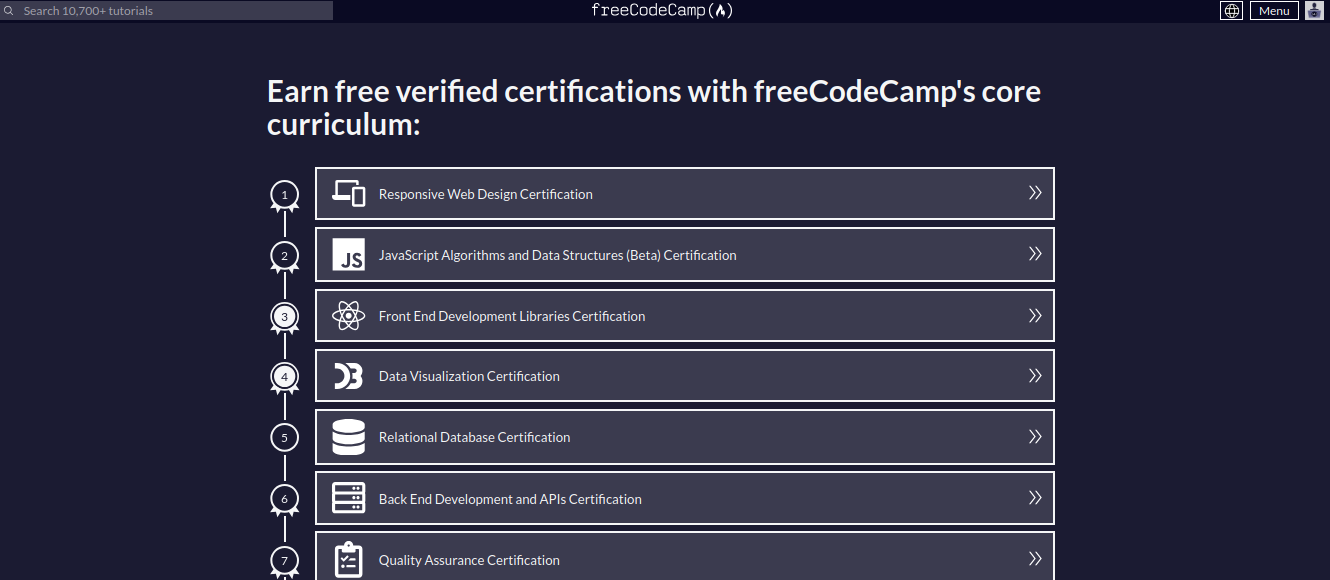
\includegraphics[width=0.6\textwidth]{pages/images/freecodecamp2.png}
    \caption[Figure 1:]{Présentation des cours du plateforme FreeCodeCamp}\label{fig:test}%
  \end{figure}
  \newline
\textbf{HackerRank}
 est une entreprise spécialisée dans les concours de programmation pour développeurs et entreprises.
 \\Les concours de programmation d'HackerRank utilisent une multitude de langages (Java, C++, PHP, SQL, etc. ) et couvrent de nombreux domaines de l'informatique.

\begin{figure}[ht]%
    \center%
    
\includegraphics[width=0.6\textwidth]{pages/images/hackeRrank.png}
    \caption{Présentation du plateforme HackerRank}\label{fig:test}%
  \end{figure}
\subsection{Critique de l'existant}
FreeCodeCamp et HackerRank sont deux plateformes d'E-learning. On a eu
l’opportunité d’y accéder en tant que tuteur et étudiant afin de découvrir ses différends
fonctionnalités.
\\
Plusieurs insuffisances ont été détectées à savoir ;
\begin{itemize}
    
\item  Une défaillance de l’ergonomie
\item L’absence du du controle simultané, on y trouve plutôt des exercies standards 
\item  Pas d’espace réservé pour les exercices demandés ou les apprenants peuvent échanger des exercices entre eux et pas d’indexation sur les exercices présents sur la plateforme.
\item Absence d’une matrice des experts selon leurs compétences qui permet à l’apprenant
de consulter leurs coordonnées.

\begin{figure}[ht]%
    \center%
    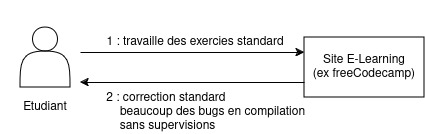
\includegraphics[width=0.8\textwidth]{pages/images/porblem.jpg}
    \vspace{3mm}
    \caption{Présentation du problématique}\label{fig:test}%
  \end{figure}

\vspace{10mm}
\subsection{Solutions proposé}
La solution que nous proposons consiste à concevoir et développer une plateforme
baptisée au sein InnoThink Académie nommée CodeNest . Cette application offre plusieurs volets comme l’E-Learning, Blended Learning, Social Learning et mobile Learning.
\begin{itemize}
    \item Knowledge-Base : C’est une base de documents confidentiels de InnoThink
consultables non téléchargeables.
\item Expert-Base : C’est une base des experts qui vont générer une liste de support de cours contenant des exercices 
\end{itemize}
Par ailleurs CodeNest  est une plateforme de partage de
connaissances entre les différents collaborateurs et sert aussi de référentiel pour le suivi des
parcours de compétences et de carrières pour les collaborateurs.
\vspace{5mm}
\begin{figure}[ht]%
    \center%
    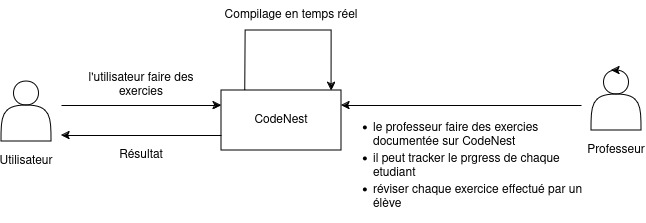
\includegraphics[width=1\textwidth]{pages/images/asma-solution.jpg}
    \vspace{3mm}
    \caption{Présentation de la solution proposée}\label{fig:test}%
  \end{figure}

\section{Méthodologie de travail et formalisme des modelisations}
Dans cette partie, nous allons définir la méthode de travail ainsi que le choix d'utilisation
\subsection{Language de modelisation}
L'UML (Unified Modeling Language) est la  Langage de modélisation unifié, et un langage de modélisation graphique est une méthode normalisée qui permet de présenter les besoins du projet sous forme de diagramme .
\\À noter que l'UML n'est pas une méthode mais une démarche qui se base sur une approche objet:
\\UML possède 3 principes fondamentaux :
\begin{itemize}
\item Guidée par les besoins du client;
\item Basé sur le diagramme de classes où on trouve les différentes entités avec les
attributs et les différentes fonctionnalités et les autres diagrammes nous permettent
d’avoir une vue détaillée sur les besoins
\item démarche itératif et incrémental
\end{itemize}
% \vspace{10mm}
\subsection{Méthodologie de travail}
{\bf{Méthode agile:}}
Le plateforme que nous souhaitons développer est à la fois dynamique et complexe, et que notre domaine d'activité est l'éducation ainsi que  la méthodologie la plus conseillée est le Scrum.
L'interaction entre l'équipe de développement, les consultants et le client est un aspect crucial dans la méthodologie agile.

\vspace{8mm}

{\bf{ Scrum :}}est un framework ou cadre de développement complexe qui est conçu pour aider les équipes à travailler ensemble de manière plus efficace et productive.

La figure représente les principales étapes de la méthodologie Scrum, chacune d'entre eux implique de différents processus à suivre.
\begin{figure}[H]%
    \center%
    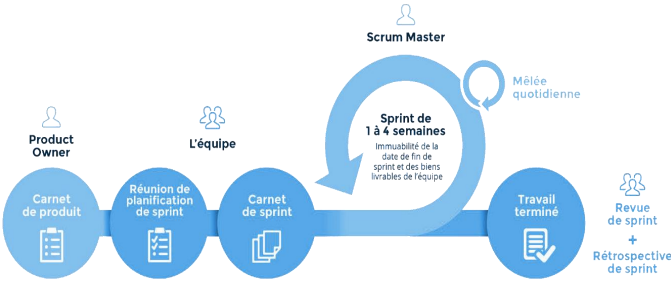
\includegraphics[width=0.6\textwidth]{pages/images/scrum.png}
    \caption{La méthodologie Scrum}\label{fig:test}%
  \end{figure}

\vspace{8mm}

 {\bf{ Sprint :}}La planification du sprint comprend l’identification des points prioritaires que l’équipe pense pouvoir réaliser au cours du sprint.

La revue du sprint a lieu à la fin de chaque sprint où l’équipe de développement présente les fonctionnalités terminées. L’incrément produit est éventuellement livrable et la mise en place du prochain sprint peut être anticipée.



  
\subsection{Choix de la méthode}
Nous avons choisi d’utiliser la méthode de SCRUM afin de gérer notre projet. Cette
méthode va nous permettre, en cas de besoin, d’ajouter ou de modifier des fonctionnalités au
niveau d’un sprint désiré sans affecter les autres. En plus, cette méthode nous permettra
de mieux respecter les dates planifiées pour clôturer les différents sprints.






 


\section{Conclusion}
Ce chapitre commence par la présentation du cadre global de notre projet,
en exposant l’organisation qui nous accueille, c’est la solution que nous proposons afin de minimiser la durée de formation en Innothink.
\\Dans le chapitre suivant, nous allons représenter les
différents besoins susmentionnés sous forme de diagrammes UML (Unified
Modeling Language) et de sprints.


        \clearpage


        
        %\chapter{Mise en oeuvre du projet}
        %\label{chap:2}
        % \addcontentsline{toc}{chapter}{Chapitre 2 : Mise en Ouevre de Projey } 
\section{Introduction}
Dans ce chapitre, nous allons commencer par illustrer le sprint 0 de notre projet.
Ensuite nous aurons recours aux explications des différents termes caractérisant notre projet.\\
Par la suite, nous allons définir les besoins spécifiques de notre projet, ainsi que le Backlog Produit permettant de déterminer les fonctionnalités de base de ce projet selon la difficulté et la priorité. En addition, nous allons présenter les outils utilisés, illustrer l’architecture et établir le diagramme de cas d’utilisation.

\section{Spécification des besoins}
Les besoins fonctionnels et non fonctionnels feront le but de cette partie ce qui nous permettra de concevoir les objectifs de InnoThink.

La phase d’analyse est primordiale dans le cycle de développement d’une application
afin de bien répartir le projet sur des sprints comme l’indique la méthodologie SCRUM.
\subsection{Identification des acteurs}
\begin{comment}
\begin{table}[h!]
    \centering
    \begin{tabular}{|l|l|l|}
        \hline
        \textbf{Acteur} & \textbf{Type Acteur} & \textbf{Description} \\
        \hline
        \multirow{4}{*}{Utilisateur} & Acteur Principal (physique) & Authentifier, Connecter au VPN, Joindre un réseau, Créer un réseau \\
        \cline{2-3}
        & & Modifier un réseau, Supprimer un réseau, Supprimer un utilisateur, Modifier un utilisateur, Créer un utilisateur \\ 
        \hline
        \multirow{5}{*}{Serveur-Web} & Acteur Secondaire (moral) & Enregistrer chaque modification d’un utilisateur dans la base de données \\
        \cline{2-3}
        & & Enregistrer chaque modification d’un réseau dans la base de données \\
        \cline{2-3}
        & & Joindre l’utilisateur dans un réseau \\
        \cline{2-3}
        & & Créer le nouveau réseau de l’utilisateur \\
        \cline{2-3}
        & & Rassembler chaque utilisateur dans un réseau privé \\
        \hline
        \multirow{3}{*}{Serveur-VPN} & Acteur Secondaire (moral) & Transmet le trafic au utilisateur \\
        \cline{2-3}
        & & Donne une adresse publique à l’utilisateur \\
        \cline{2-3}
        & & Donne une adresse privée à l’utilisateur \\
        \hline
    \end{tabular}
    \caption{Description des acteurs}
    \label{tab:acteurs}
\end{table}
\end{comment}









\textbf{L’admin: }L’acteur principal qui a le rôle le plus important de gèrer l’administration de la plateforme.


\textbf{Le visiteur:} L’acteur secondaire qu’il va découvrir les cours de la plateforme sans s’authentifier.


\\ \textbf{Collaborateur:} L’acteur qui va utiliser les services de la plateforme.


\\ \textbf{Formateur:} L'acteur celui qui va déposer un support de cours


\subsection{Les besoins fonctionnels}
Les exigences fonctionnelles de notre solution sont classées selon les acteurs
impliqués.ainsi que l'assignation des rôles à chaque utilisateur.


\textbf{Gestion des accès à la plateforme :} Cela inclut la création, la modification, la suppression des comptes
\textbf{Gestion des exercies :}Ce module inclut le dépôt des exercies , leur modification et leur suppression.

 
\textbf{Gestion des avis:}  Cela inclut l'ajout, la modification et la suppression des avis.   

\vspace{9mm}

\textbf{Gestion des utilisateur :} Cela inclu , la modifications et la suppression des données des utilisateurs ( étudiant ou professeur ) 




\subsection{Les besoins non fonctionnels}

Les exigences non fonctionnelles définissent le comportement et la performance que le produit doit présenter.
\begin{itemize}
\item \textbf{La performance :} Il est essentiel que la plateforme soit rapide et réactive, garantissant une expérience utilisateur fluide même lorsqu'il y a un grand nombre d'utilisateurs en même temps.

\item \textbf{La sécurité: }La sécurité des donnés des utilisateurs est essentielle ou il doit utiliser des protocoles de cryptage afin de préserver les informations confidentielles telles que les identifiants de connexion et les informations d’authentification

\item \textbf{La disponibilité :}Il est essentiel que la plateforme soit accessible tous les 24 heureset les 7 jours, avec un temps d'arrêt minimal afin de garantir l'accès au cours et aux ressources à tout moment.

\item \textbf{La facilité:} La plateforme devrait être facile à utiliser, avec une interface intuitive et des instructions claires pour faciliter la navigation et l'utilisation des cours et des ressources disponibles.

\item \textbf{Accessibilité :}  La plateforme doit être accessible à tous les utilisateurs, y compris ceux qui ayant des besoins spécifiques en matière d'accessibilité.
\end{itemize}

\newpage
\subsection{Backlog produit}

	\begin{table}[H] % Changed to table for single-column layout
	    \centering
	    \begin{tabular}{|p{3cm}|p{1.5cm}|p{7cm}|p{1.3cm}|}
	        \hline
	        Spirnt & ID User Story & User Story & Priorité \\
	        \hline
	        Gestion d'accès de la plateforme & 1.1 & En tant que visiteur je veux m'inscrire & 3 \\ \hline
        & 1.2 &  En tant que étudiant je veux m’authentifier & 4 \\ \hline 
        & 1.2 &  En tant que professeur je veux m'authentifer  mon compte & 4 \\ \hline 
        & 1.2 &  En tant que admin je veux m'authentifier & 4 \\ \hline 
		









        Gestion des exercices 
        & 2.1 &  En tant que visiteur je veux consulter les exercies & 3 \\ \hline
        & 2.1 &  En tant que étudiant je veux chercher un exercises & 3 \\ \hline
        & 2.1 &  En tant que étudiant je veux m’inscrire à un series des exercies & 3 \\ \hline
        & 2.1 &  En tant que étudiant je veux consulter le progrès des exercies & 3 \\ \hline
        & 2.1 &  En tant que professeur je veux déposer un ou des exercies & 3 \\ \hline
        & 2.1 & En tant que professeur je veux supprimer un exercies & 3 \\ \hline
        & 2.1 & En tant que administrateur je veux consulter un exercies & 3 \\ \hline
        & 2.1 & En tant que administrateur je veux déposer un exercies & 3 \\ \hline
        & 2.1 & En tant que administrateur je veux supprimer un exercies & 3 \\ \hline












        Gestion des avis & 3.1 &  En tant que visiteur je veux consulter les avis & 9 \\ \hline
        & 3.2 &  En tant que étudiant je veux consulter les avis & 10 \\ \hline
        & 3.3 &  En tant que étudiant je veux donner un avis & 10 \\ \hline
        & 3.4 & En tant que professeur je veux consulter les avis & 10 \\ \hline	
        & 3.5 & En tant que professeur je veux donner un avis & 10 \\ \hline
        & 3.5 & En tant que admin je veux consulter les avis & 10 \\ \hline
        & 3.5 & En tant que admin je veux supprimer un avis & 10 \\ \hline










     
    \end{tabular}
    \caption \centering{Backlog produit globale}
    \label{tab:my_label}
	\end{table}











	\begin{table}[H] % Changed to table for single-column layout
	    \centering
	    \begin{tabular}{|p{3cm}|p{1.5cm}|p{7cm}|p{1.3cm}|}
	        \hline
	        Spirnt & ID User Story & User Story & Priorité \\
	        \hline
            Gestion des utilisateurs  & 4.1 & en tant que administrateur je veux consulter les utilisateurs de la platform & 9 \\ \hline
        & 4.2 & en tant que administrateur je veux créer un nouveau utilisateur & 10 \\ \hline
        & 4.3 & en tant que administrateur je veux modifier les utilisateurs & \\ \hline
        & 4.3 & en tant que administrateur je veux supprimer des utilisateurs & \\ \hline
    \end{tabular}
    \caption \centering{Backlog produit globale}
    \label{tab:my_label}
	\end{table}








\subsection{Diagramme de cas d'utilisation globale}
\\
Chaque interaction entre les utilisateurs et le système est définie comme un cas d'utilisation.
Chaque cas d'utilisation représente une fonctionnalité offerte aux utilisateurs pour atteindre un résultat spécifique. Le diagramme de cas d'utilisation décrit donc cette interaction en identifiant les besoins de l'utilisateur et toutes les actions que le système doit effectuer pour répondre à ces besoins.

%DIAGRAMME DE CAS D UTILISATION
  \begin{figure}[h]%
    \center%
    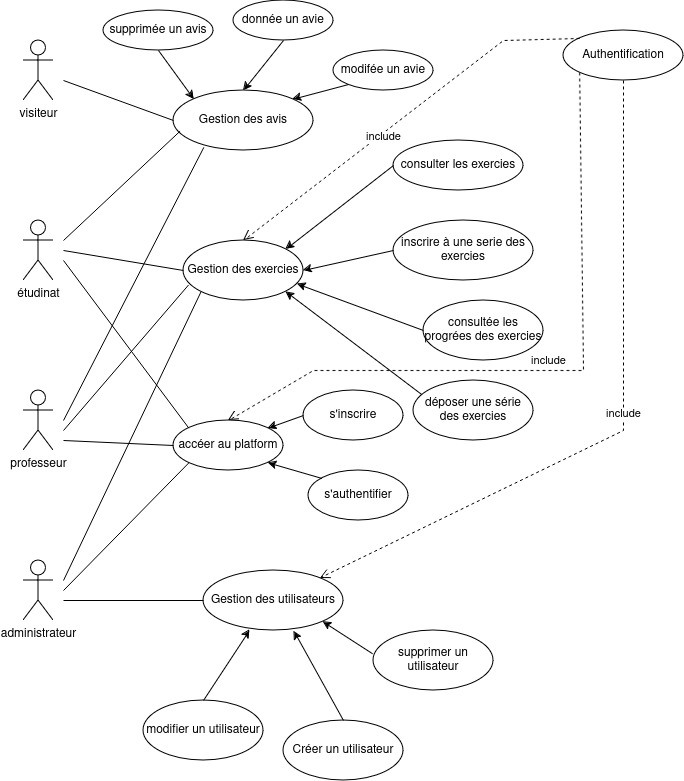
\includegraphics[width=0.6\textwidth]{pages/image/asma-usecase-global.jpg}
            \caption{pésentation de diagramme de cas d'utilisation}\label{fig:test}%
  \end{figure}

\section{Planification des sprints:}
 \subsection{\normal \series{ Sprint1: }Gestion d'accès de la plateforme}
Dans ce sprint, nous nous concentrerons sur la présentation de la manière dont nous avons réussi à mettre en place la gestion d'accès sur la plateforme en utilisant des techniques d'authentification. Nous énumérerons également les technologies utilisées pour créer une page de connexion et d'inscription adaptée et présentable. De plus, nous montrerons comment un utilisateur peut modifier certaines informations de son compte .
 
 \subsection {\normal \series{ Sprint2: }Gestion des exercises}
 Dans ce sprint, nous présenterons le processus de création d'une interface permettant aux utilisateurs d'accéder aux exercices fournis par le créateur des exercices (le professeur). Nous montrerons également comment compiler ces exercices en temps réel et stocker les résultats dans une base de données.
 
 \subsection {\normal \series{Sprint3: }Gestion des avis}
Ce sprint est principalement axé sur la fourniture aux utilisateurs de la possibilité de consulter la note des exercices en fonction des évaluations d'autres personnes à l'aide d'un système de notation. De plus, les utilisateurs pourront attribuer une note, la modifier et la supprimer après avoir terminer un exercice.

 \subsection {\normal \series{Sprint4: }Gestion des utilisateurs}
Ce chapitre se concentre sur la manière dont l'administrateur du site web interagit avec les utilisateurs et le contenu du site. L'administrateur a la capacité de manipuler (modification, supprission) des utilisateurs ou des exercices.















\section{Étude technologiques}
Dans cette partie, nous allons définir environnement matériel ainsi
que l’environnement logiciel afin d’élaborer ce projet.
\subsection{Environnement matériel}  
Cette plateforme a été développée avec un ordinateur Lenovo ayant les caractéristiques suivante:
\begin{itemize}
    \item  Processeur Dual Core AMD Athlon Silver 3050U   
      \item  Mémoire 12 Go
    \item Disque 512 Go SSD NV Me
    \item Carte graphique AMD Radeon Graphics Intégré 
\end{itemize}

\subsection{Environnement Logiciel}
 {\bf{ Visual Studio Code:}}
 Visual Studio Code est un éditeur de code open-source développé par Microsoft. Léger et puissant, il supporte de nombreux langages de programmation et offre des fonctionnalités telles que l'autocomplétion, le débogage et l'intégration Git. Avec ses extensions, VS Code s’adapte facilement aux besoins des développeurs.
 \begin{figure}[H]%
    \center%
    
\includegraphics[width=0.3\textwidth]{pages/images/vscode.png}
    \caption{ Logo Visual Studio Code}\label{fig:test}%
  \end{figure}

\vspace{10mm}
 {\bf{Postman :}}
 Postman est un outil populaire utilisé pour tester et interagir avec des APIs. Il permet de créer, envoyer et gérer des requêtes HTTP de manière simple et intuitive. Avec Postman, vous pouvez inspecter les réponses des APIs, automatiser les tests, et gérer des environnements de développement. C’est un outil essentiel pour les développeurs et les testeurs qui travaillent avec des services web et des interfaces de programmation.
 \begin{figure}[H]%
    \center%
    
\includegraphics[width=0.25\textwidth]{pages/images/postman.png}
    \caption{Logo Postman}\label{fig:test}%
  \end{figure}
 




{\bf{Mongo DataBase :}}
MongoDB est une base de données NoSQL orientée documents. Contrairement aux bases de données relationnelles, MongoDB stocke les données en format BSON (Binary JSON), ce qui permet une flexibilité accrue dans la gestion des données semi-structurées et non structurées. 
\\
Il est conçu pour évoluer horizontalement, facilitant ainsi la gestion de grandes quantités de données. MongoDB est apprécié pour sa performance, sa scalabilité et sa capacité à s'adapter aux besoins variés des applications modernes.
 \begin{figure}[H]%
    \center%
    
\includegraphics[width=0.3\textwidth]{pages/images/mongo.png}
    \caption{ Logo Mongo Data base}\label{fig:test}%
  \end{figure}





{\bf{Github :}}
GitHub est une plateforme de gestion de code source basée sur Git, qui facilite la collaboration entre développeurs.
\\
Elle permet de stocker et de suivre les versions du code, de gérer les projets avec des fonctionnalités telles que les demandes de tirage (pull requests), les issues, et les wikis.
\\
GitHub offre également des outils pour la collaboration en équipe, comme les revues de code et les intégrations continues, rendant le développement logiciel plus fluide et organisé.
 \begin{figure}[ht]%
    \center%
    
\includegraphics[width=0.25\textwidth]{pages/images/GitHub.png}
    \caption{ Logo Github}\label{fig:test}%
  \end{figure}







{\bf{Figma :}}
Figma est un outil de conception d'interface utilisateur et de prototypage collaboratif basé sur le cloud.
\\
Il permet aux designers de créer des maquettes interactives et des prototypes en temps réel tout en facilitant la collaboration entre les membres d'une équipe.
 Sa nature collaborative et ses fonctionnalités de versioning rendent le processus de conception plus fluide et intégré.
 \begin{figure}[H]%
    \center%
    
\includegraphics[width=0.3\textwidth]{pages/images/figma-1698087967030-2x.jpg}
    \caption{ Logo Figma }\label{fig:test}%
  \end{figure}





\subsection{Technologie et langage utilisée }
 {\bf{ ReactJS:}}
Est une bibliothèque JavaScript développée par Facebook pour la création d'interfaces utilisateur. Elle permet de construire des applications web dynamiques et réactives grâce à une approche basée sur des composants réutilisables. React utilise un DOM virtuel pour optimiser les mises à jour de l'interface, ce qui améliore les performances. Avec sa syntaxe JSX et son écosystème riche, ReactJS facilite le développement d'applications modernes et interactives.
 \begin{figure}[H]%
    \center%
    
\includegraphics[width=0.3\textwidth]{pages/images/react.png}
    \caption{ Logo ReactJS}\label{fig:test}%
  \end{figure}

 {\bf{ TypeScript:}}
Est un langage de programmation développé par Microsoft qui est une surcouche de JavaScript. Il ajoute des types statiques optionnels au langage, ce qui permet de détecter les erreurs de type lors de la compilation plutôt qu'à l'exécution. TypeScript offre également des fonctionnalités avancées comme les classes et les interfaces, facilitant ainsi le développement d'applications robustes et maintenables. Il se compile en JavaScript, ce qui permet une intégration facile avec les projets JavaScript existants.
 \begin{figure}[H]%
    \center%
    
\includegraphics[width=0.2\textwidth]{pages/images/typescript.png}
    \caption{ Logo TypeScript }\label{fig:test}%
  \end{figure}






 {\bf{ NodeJS:}}
 Est un environnement d'exécution JavaScript côté serveur, basé sur le moteur V8 de Google Chrome. 
\\
Il permet aux développeurs d'utiliser JavaScript pour écrire des scripts côté serveur, ce qui facilite le développement d'applications web évolutives et performantes. 
\\
Nodejs est réputé pour sa gestion efficace des opérations asynchrones et son architecture événementielle, ce qui le rend idéal pour les applications en temps réel comme les chats et les jeux en ligne. Avec un vaste écosystème de modules via npm, Node.js offre de nombreuses bibliothèques et outils pour enrichir vos projets.
 \begin{figure}[H]%
    \center%
    
\includegraphics[width=0.25\textwidth]{pages/images/nodejs.png}
    \caption{Logo NodeJS}\label{fig:test}%
  \end{figure}

 {\bf{ ExpressJS:}}
Express est un framework minimaliste pour Node.js, utilisé pour créer des applications web et des APIs.
\\
Il simplifie le processus de gestion des requêtes HTTP, la définition des routes, et le traitement des middleware.
\\
Express est apprécié pour sa flexibilité et sa simplicité, permettant aux développeurs de construire des applications robustes et performantes avec moins de configuration.
\\s
 \begin{figure}[H]%
    \center%
    
\includegraphics[width=0.2\textwidth]{pages/images/expressjs_logo_icon_169185.png}
    \caption{Logo Express JS}\label{fig:test}%
  \end{figure}







 {\bf{ tailwind CSS:}}
Est un framework de design utilitaire pour créer des interfaces web modernes et réactives.
Contrairement aux frameworks CSS traditionnels, Tailwind se base sur une approche de classes utilitaires qui permettent de styler directement les éléments HTML.
\\
Cette approche offre une grande flexibilité et un contrôle précis sur le design tout en évitant le besoin d'écrire des CSS personnalisés.
\begin{figure}[H]%
    \center%
    
\includegraphics[width=0.25\textwidth]{pages/images/tailwind.jpg}
    \caption{ Logo Tailwind CSS}\label{fig:test}%
  \end{figure}






\section{Justification des choix technologiques}
Le choix de React pour le front-end et Node.js pour le back-end s'appuie sur leur capacité à offrir des performances optimales, une modularité accrue, et une intégration fluide dans une plateforme éducative en ligne. React permet de créer des interfaces utilisateur dynamiques et réactives, avec une structure de composants réutilisables qui facilite le développement et la maintenance. Node.js, de son côté, assure une unification du langage JavaScript sur toute la stack, simplifiant la communication entre le front-end et le back-end et permettant de gérer efficacement un grand nombre de connexions simultanées, ce qui est essentiel pour une plateforme éducative évolutive et performante.






















\section { Conclusion}
\\
Dans ce chapitre, j’ai présenté le product Backlog et le diagramme global enfin j’ai présenté les logiciels et les langages utilisés dans le chapitre suivant, je vais présenter la première realisation.















        \clearpage


        % \chapter{Sprint 1: Gestion d'accées de la plateforme}
        % \label{chap:3}
        % 
\usepackage{float}
\addcontentsline{toc}{chapter}{Chapitre 3 : Introduction générale} 
\section{Introduction:}
Nous allons, dans ce chapitre, analyser et détailler le premier Sprint qui a pour but de réaliser la partie Authentification et la  sécurité . Ainsi que les différents stories. En premier lieu, nous présentons le backlog du Sprint
contenant l’ensemble des tâches à réaliser. Ensuite, nous allons raffiner les besoins et entamer la solution conceptuelle en exposant les différents diagrammes qui décrivent l’interactionentre le système et l’utilisateur afin d’atteindre le résultat désiré.
\section{Backlog Sprint1 }
Ce tableau représente le premier module du premier Sprint ainsi que les différents User Story.








\begin{table*}[h]
    \begin{center} 
    \begin{tabular}{|p{3cm}|p{5cm}|p{3cm}|p{1.9cm}|p{2cm}|} \hline 
          Module &  User Stories &  Tache &  Complexité & Estimation \\ \hline

            Gestion d'accé de la plateforme & En tant que visiteur je veux m'inscrire   & - Dévelopement du backend & \centering L & 1 jour  \\  \hline

            & En tant que étudiant je veux m’authentifier & & \centering L & 1 jour   \\ \hline
            & En tant que professeur je veux m'authentifer mon compte& & \centering  L & 1 jour   \\ \hline
            & En tant que admin je veux m'authentifier & & \centering  L & 1 jour   \\ \hline
           




       
    \end{tabular}
  \end{center}
  \center
  \caption { Backlog sprint1}
\label{tab:bert_res}
\end{table*}  




\section{Analyse fonctionnelle}
Dans cette partie on va présenter les besoins fonctionnels qui seront répartis suivant 2 modules à savoir :



\begin{itemize}
    \item \textbf{S'authetifier:} l'utilisateur va s'authentifier au plateforme après entrer ses coordonnés corrects.

    \item \textbf{S'inscrire}  : l'utilisateur va créer un compte pour accéder aux services et fonctionnalités après fournir les informations nécessaires qui sont "username" "email" et "password".


    

   
\end{itemize}
\section{Raffinement du sprint 1}
\subsection{Rafinnement de cas d'utilisation "Authentification"}
L’authentification est le besoin primordial pour le traitement et la sécurité des autres cas d’utilisation.
Pour que les utlisateurs qui sont un collaborateur, un formateur ou un admin  puissent exécuter leurs propres besoins, ils sont obligés de passer par l’authentification.
cette figure nous illustre le diagramme de cas d’utilisation « S’authentifier » :


\begin{figure}[!h]
\center
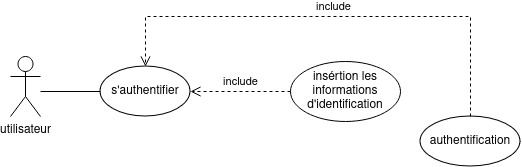
\includegraphics[width=0.8\textwidth]{pages/image/asma-usecase-authenthification.jpg}
\caption{Présentation de cas d'utilisation"s'authentifier"}
\end{figure}


\subsubsection{Déscription textuelle}  

\begin{table*}[h]
    \begin{center} 
    \begin{tabular}{|p{4cm}|p{9cm}|}  \hline 
       Cas d'utilisation& Authentification \\ \hline
       Acteur&collaborateur, formateur, admin \\ \hline
       Précondition&  L’utilisateur doit être enregistré dans la base
       de données      \\ \hline
       Post condition& L’utilisateur peut accéder aux différentes fonctionnalités du plateforme \\ \hline
       Scénario nominale&Le système affiche le formulaire d’identification. \\
       &L'utilisateur entre ses informations nécessaire pour s'authentifier.\\
          & Le systéme verifie les informations saisie par l'utilisateur et l'envoie vers la page d'acceuil .\\ \hline
       Scénario alternatif&      
        L'utilisateur saisie des données inncorrecte \\
         & L'utilisateur n'est pas enregistré au base de donnés \\
         & Un probléme de connexion.
          
     \\ \hline
  \end{tabular}
  \end{center}

  \caption{ Déroulement de cas d'utilisation d'authentification}
\label{tab:bert_res}
\end{table*}



















\subsection{Rafinnement de cas d'utilisation "S'inscrire"}
La figure 19 nous illustre le diagramme de cas d’utilisation « S’inscrire » :

\begin{figure}[!h]
\center%
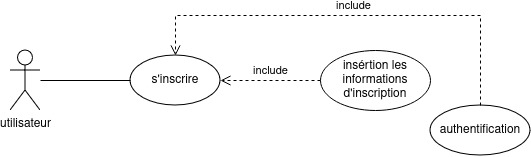
\includegraphics[width=0.8\textwidth]{pages/image/asma-usecase-inscrire.jpg}
\caption{Diagramme du cas d'utilisation "Inscrire"}
\end{figure}


\subsubsection{Déscription textuelle}  

\begin{table*}[h]
    \begin{center} 
    \begin{tabular}{|p{4cm}|p{9cm}|}  \hline 
       Cas d'utilisation& Inscrire \\ \hline
       Acteur&Visiteur,Etudiant,Admin,professeur \\ \hline
       Précondition& Connexion à l'internet   
       \\ \hline
       Post condition& L’utilisateur peut accéder aux différentes fonctionnalités du plateforme
       \\ \hline


       
       Scénario nominale& 
            L'utilisateur accéde à la page d'identification et fait l'inscription.\\
          &L'utilisateur entre ses informations nécessaire pour s'inscrire.\\
          & Le systéme verifie les informations saisie par l'utilisateur et l'envoie vers la page d'acceuil .
                       \\ \hline
                       
       Scénario alternatif&      
        L'utilisateur saisie des données inncorrecte \\
         & L'utilisateur n'est pas enregistré au base de donnés \\
         & Un probléme de connexion.
          
     \\ \hline
  \end{tabular}
  \caption{Déroulement de cas d'utilisation}
  \end{center}
\label{tab:bert_res}
\end{table*}













\section{Conception}
\subsection{Diagramme de classe  }
La figure suivant montre le diagramme de classe pour la procedure d'authentification: 
\begin{figure}[h]
    \centering
    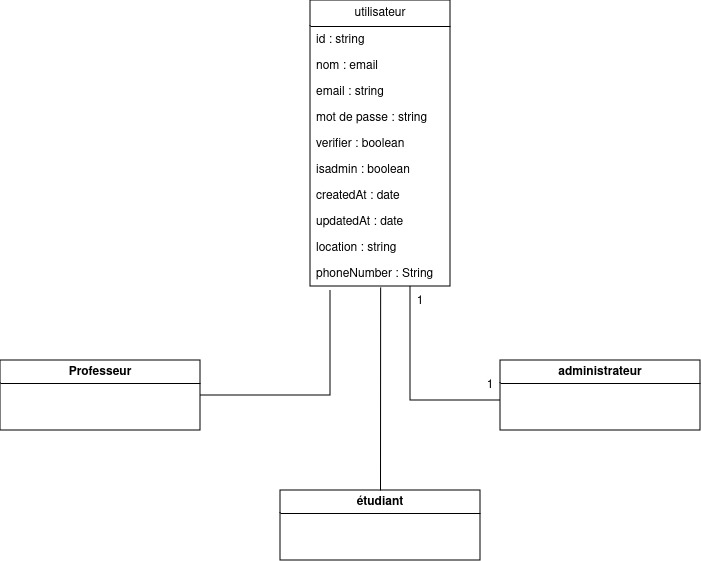
\includegraphics[width=0.65\linewidth]{pages/image/asma-class_diagramme-authentifier.jpg}
    \caption{Diagramme de classe "authentification"}
    \label{fig:enter-label}
\end{figure}

La figure suivant montre le diagramme de classe pour la procedure d'authentification: 

\begin{figure}[h!]
    \center
    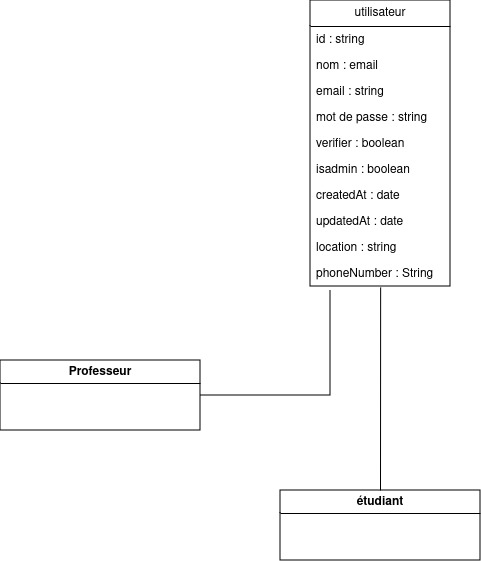
\includegraphics[width=0.5\linewidth]{pages/image/asma-classdiagramme-inscrire.jpg}
    \caption{Diagramme de classe "inscription"}
\end{figure}







\subsection{Diagramme de séquance :}
\subsubsection{Conception de partie "Authentification"}
Cette figure représente le diagramme de séquance pour l'authentification d'un utilisateur de la plateforme .\\
\begin{figure}[h!]
\center
  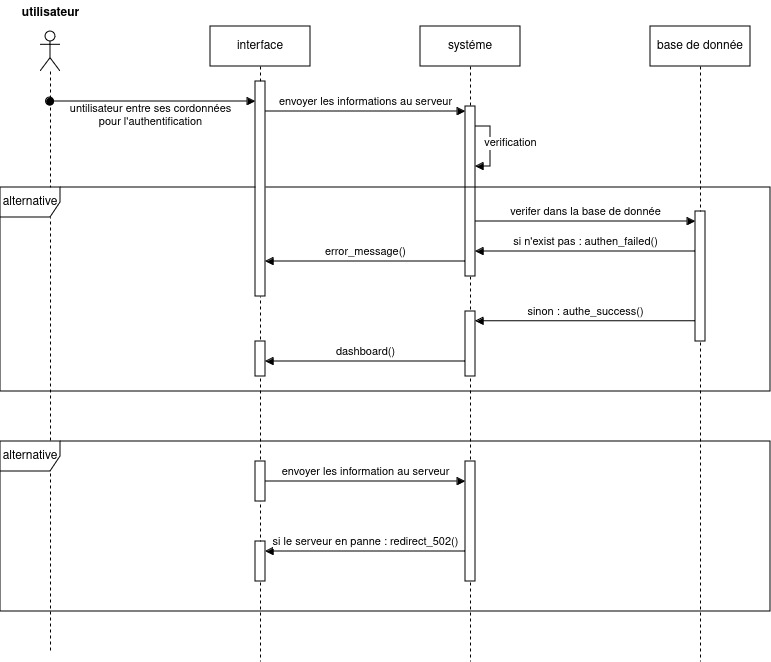
\includegraphics[width=0.6\linewidth]{pages/image/asma-diagramme_sequence-authentification.jpg}
    \caption{Diagramme de séquance  pour l'authentification d'un etudiant}
    \label{fig:enter-label}
\end{figure}




















Cette figure représente le diagramme de séquance pour l'inscription de l'utilisateur au plateforme .\\
\begin{figure}[h!]
\center
  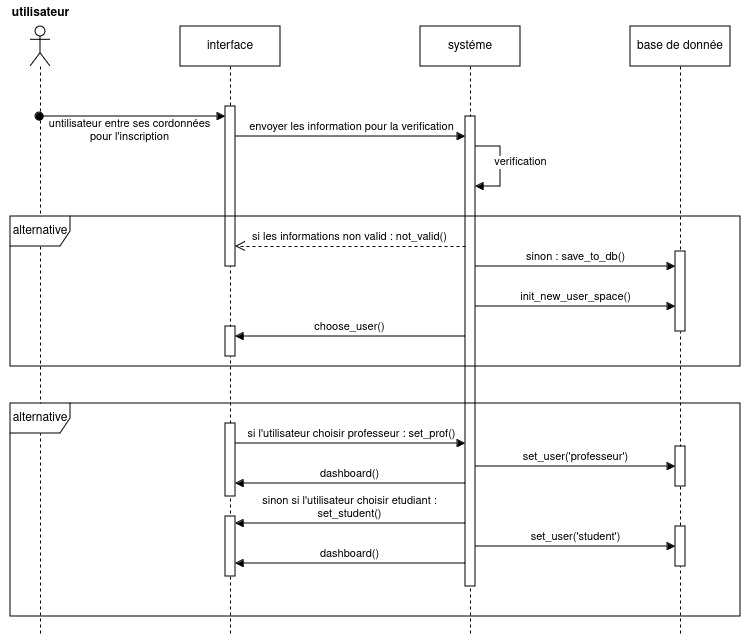
\includegraphics[width=0.65\linewidth]{pages/image/asma-diagramme_sequence-inscription.jpg}
    \caption{Diagramme de séquance  pour l'inscription d'un utilisateur}
    \label{fig:enter-label}
\end{figure}





















\subsection{Réalisation}
Dans cette section on va présenter la réalisation de l'interface pour cette chapitre.
Cette figure représente la page d'acceuil de la plateforme:
\begin{figure}[h!]
    \centering
    
\includegraphics[width=0.9
    \linewidth]{pages/images/interface1.png}
    \caption{Page d'acceuil du plateforme}
    \label{fig:enter-label}
\end{figure}
\\ 



\clearpage 
La figure suivante représante  l'interface du login et sign up  
\begin{figure}[h!]
    \centering
    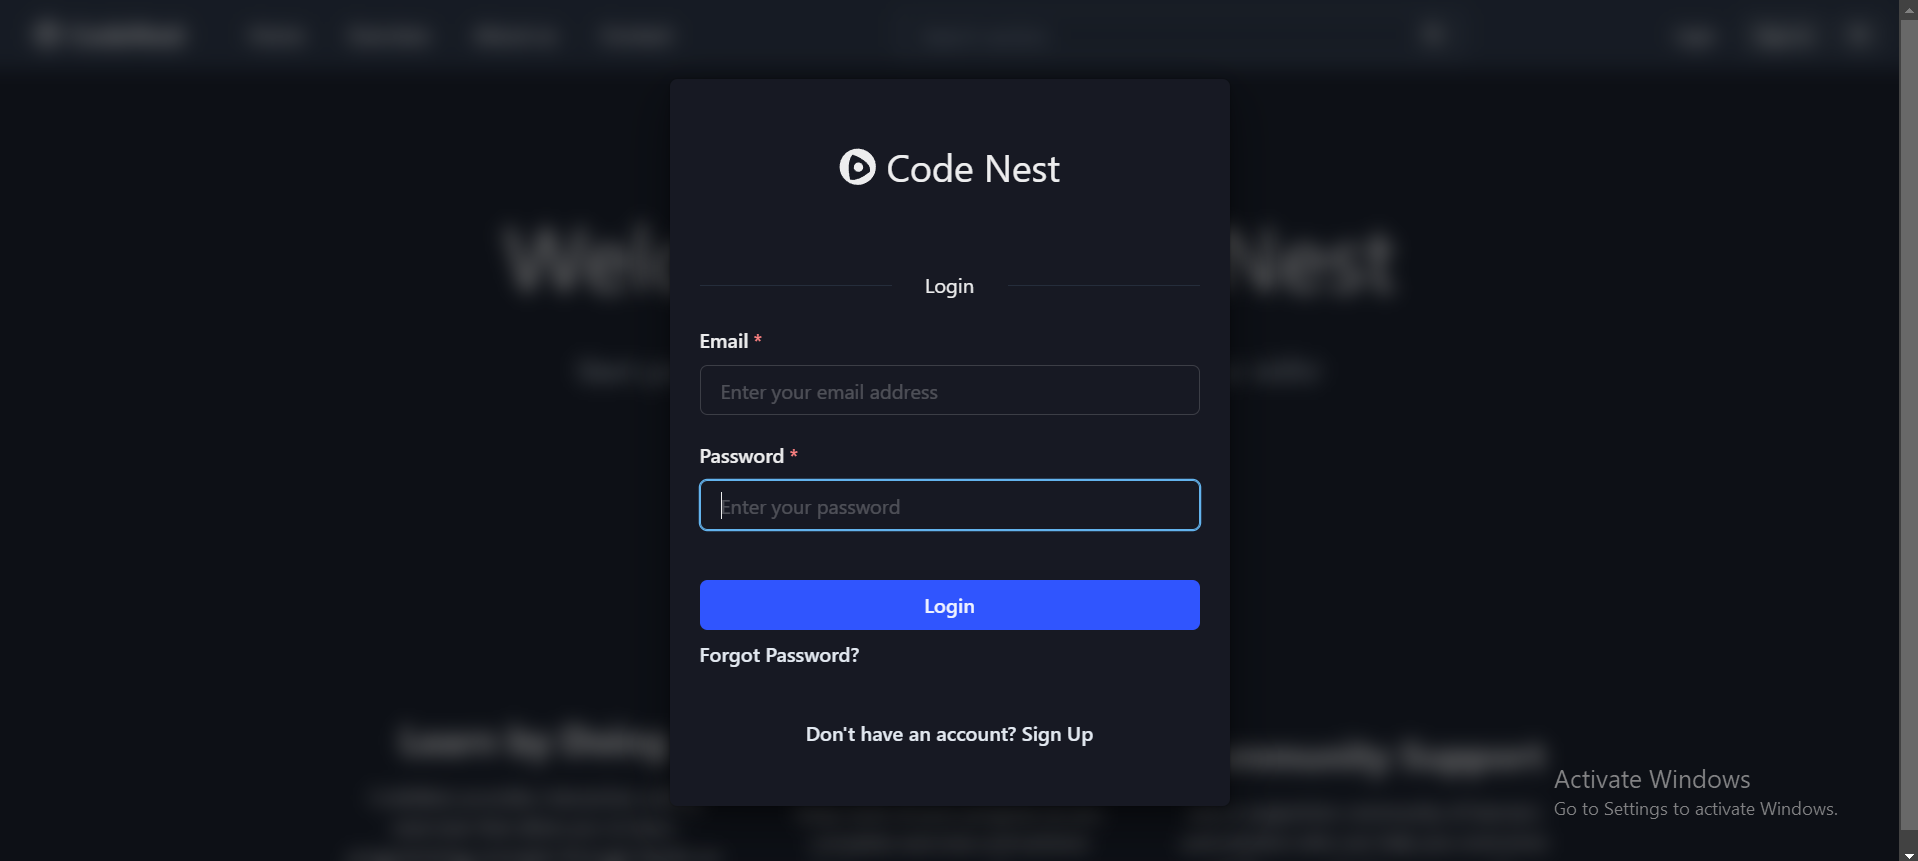
\includegraphics[width=0.9\linewidth]{pages/images/interface login.png}
    \caption{Interface du login du plateforme}
    \label{fig:enter-label}
\end{figure}


\begin{figure}[h!]
    \centering
    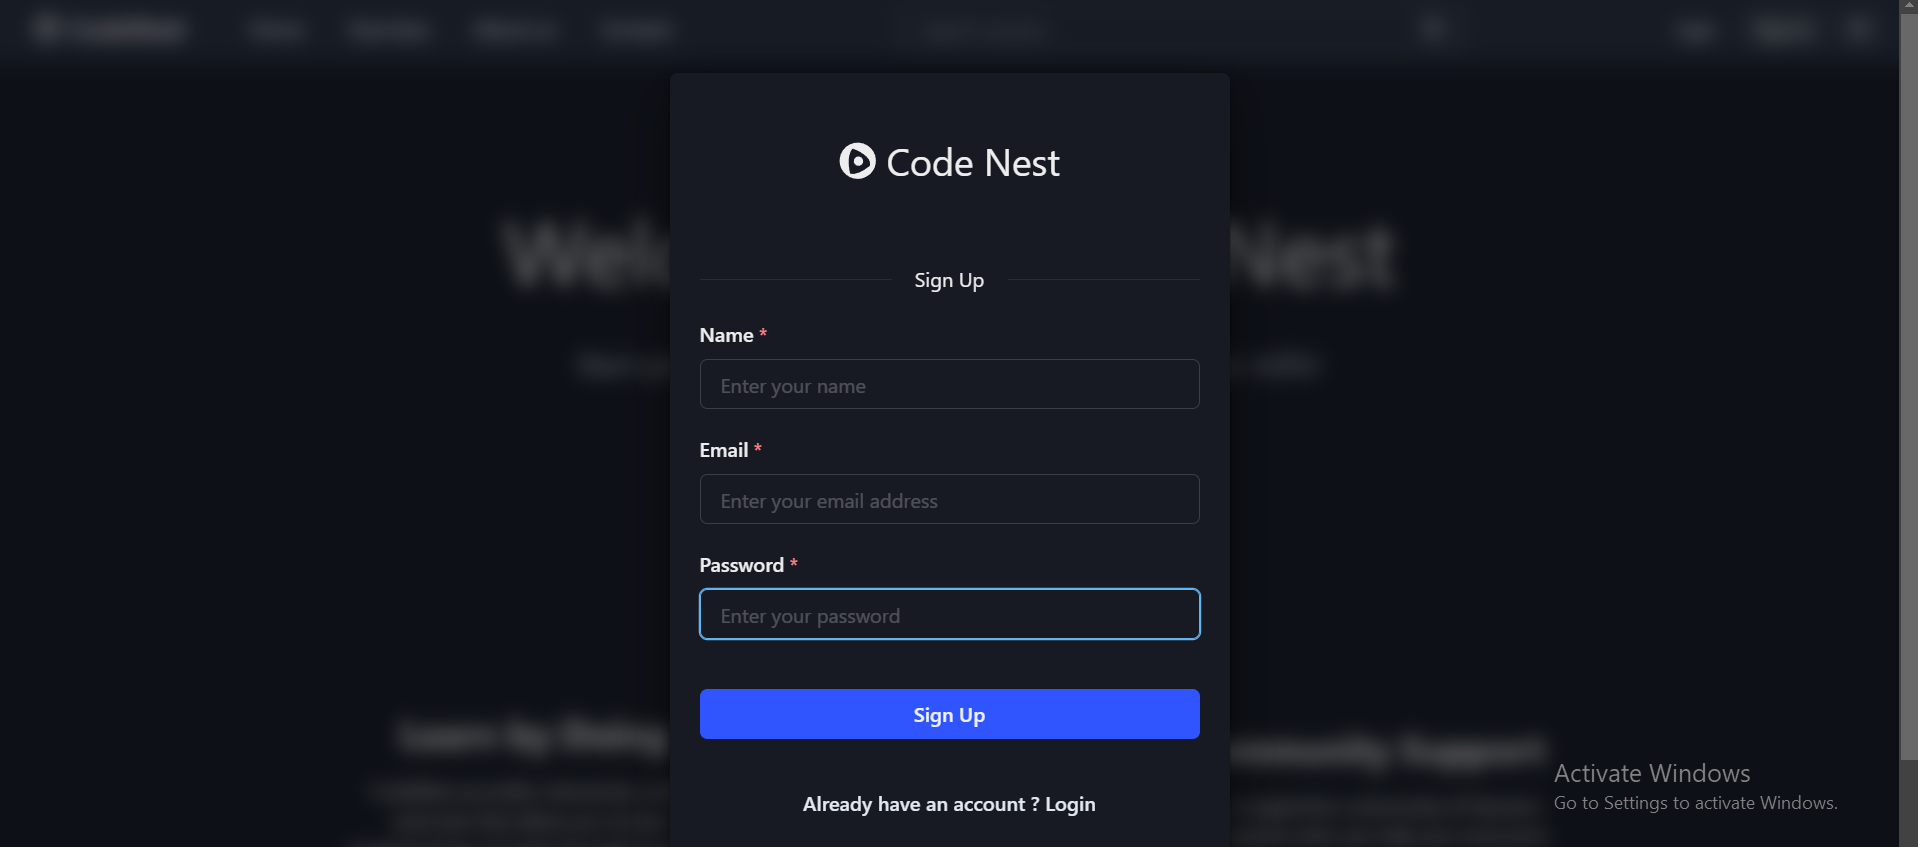
\includegraphics[width=0.9\linewidth]{pages/images/sign up interface.png}
    \caption{Interface de creation de compte du plateforme}
    \label{fig:enter-label}
\end{figure}

\clearpage
La figure montre une interface du compte  d'un utilisateur ou il peut modifier son compte
\begin{figure}[h!]
    \centering
    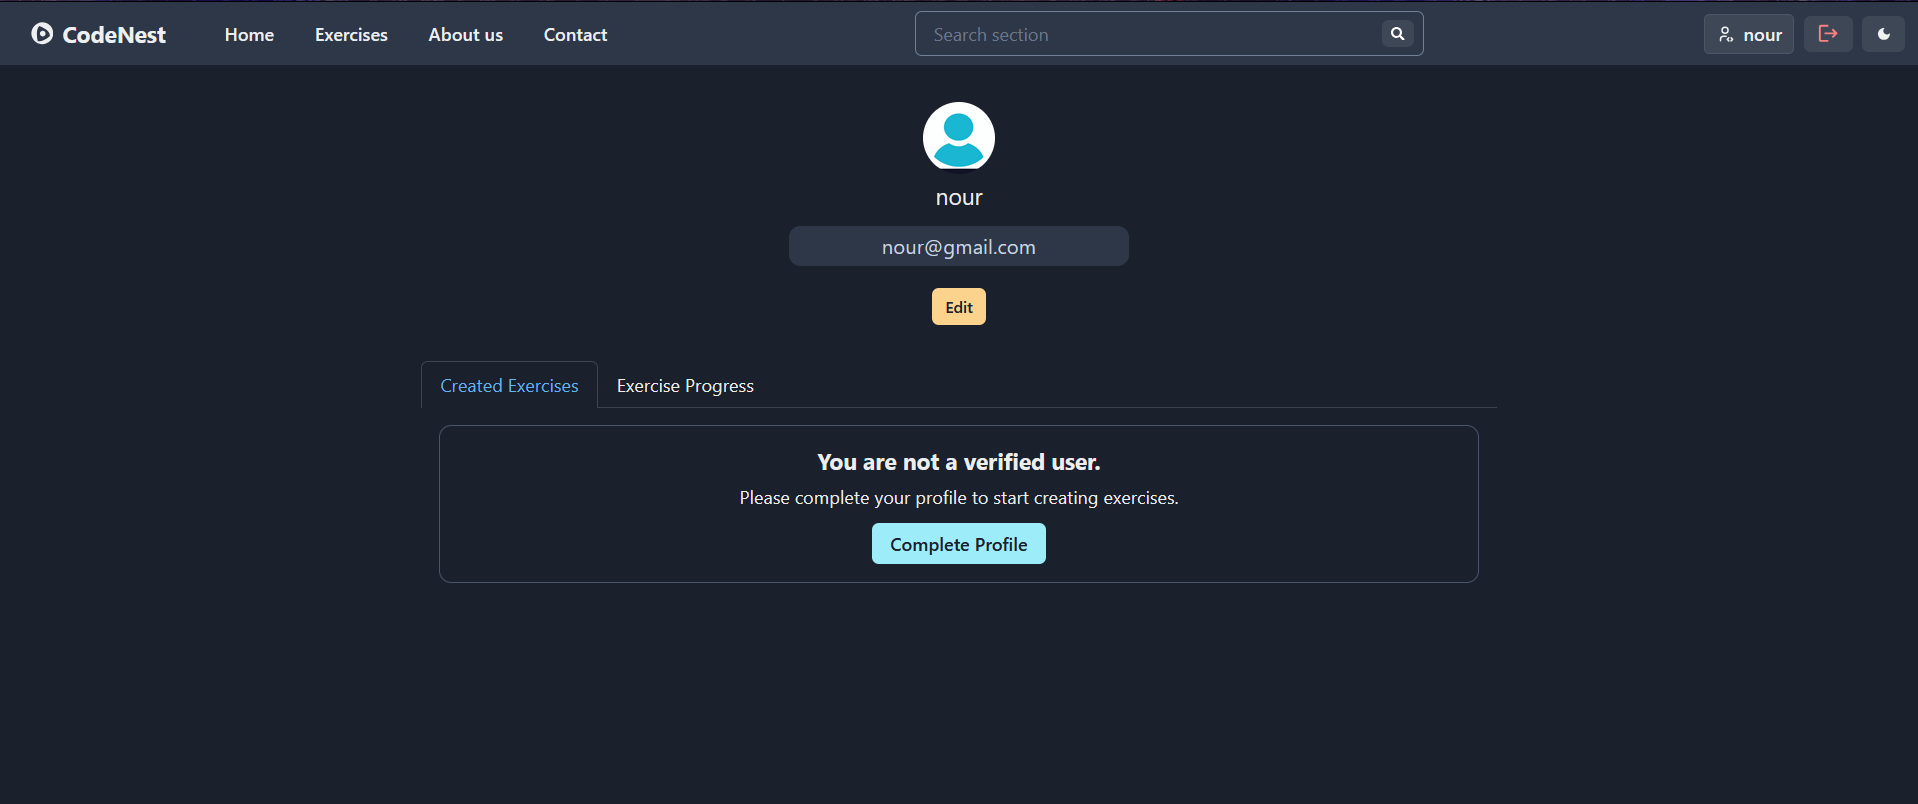
\includegraphics[width=0.9\linewidth]{pages/images/modifier compte.png }
    \caption{Interface utilisateur pour la modification du compte}
    \label{fig:enter-label}
\end{figure}
Au cas d'oublie du mot de passe l'utilisateur peut obtenir un nouveau mot de passe à travérs un email reçu contenant le nouveau code 


\begin{figure}[h!]
    \centering
    
\includegraphics[width=0.9\linewidth]{pages/images/send mail interface.png}
    \caption{Interface utilisateur pour entrer le mail }
    \label{fig:enter-label}
\end{figure}

\begin{figure}[h!]
    \centering
    
\includegraphics[width=0.9\linewidth]{pages/images/confirmation code interface.png}
    \caption{Interface  l'utilisateur de confirmation du code envoyé sur mail }
    \label{fig:enter-label}
\end{figure}


\clearpage
\section{Conclusion}
Le résultat de notre premier sprint nous permet de rassembler les données utiles pour la prochaine partie du projet. 
A cette étape on est capable de créer un Forum pour notre application web
La prochaine étape sera de traiter le second sprint qui représente une partie importante de note plateforme.
        \clearpage


        %\chapter{Sprint 2 :Gestion des exercices}
        %\label{chap:4}
        % \addcontentsline{toc}{chapter}{Chapitre 4 : Introduction générale} 
\section{Introduction}
Nous allons, dans ce chapitre, analyser et détailler le Sprint de gestions des exercies ainsi que les différents stories. 
En premier lieu, nous présentons l’organisation de ce Sprint et son Backlog que nous avons pu dégager précédemment.
Ensuite, nous allons présenter la phase d’analyse et la solution conceptuelle en exposant les différents diagrammes qui décrivent l’interaction entre le système et l’utilisateur afin d’atteindre le résultat désiré



\section{Backlog du sprint}
\begin{table*}[h]
    \begin{center} 
    \begin{tabular}{|p{2.5cm}|p{6cm}|p{2.8cm}|p{1.8cm}|p{1.8cm}|} \hline 
Module &  User Stories &  Tache &  Complexité & Estimation \\ \hline

Gestion des exercies & En tant que visiteur je veux consulter les exercies & Dévelopement du backend & \centering L & 1 jour  \\  \hline
& En tant que étudiant je veux chercher un exercises & Dévélopement backend & \centering L & 1 jour  \\ 
& En tant que étudiant je veux m’inscrire à un series des exercies & Developement du backend & &\\ \hline
& En tant que étudiant je veux consulter le progrès des exercies & Developement du backend & & \\ \hline
& En tant que professeur je veux déposer un ou des exercies  & Developement du backend & & \\ \hline
&  En tant que professeur je veux supprimer un exercies & Developement du backend & & \\ \hline
& En tant que administrateur je veux consulter un exercies & Developement du backend & & \\ \hline
&  En tant que administrateur je veux déposer un exercies & Developement du backend & & \\ \hline
& En tant que administrateur je veux supprimer un exercies & Developement du backend & & \\ \hline
\end{tabular}
\end{center}
\center
\caption { Backlog sprint 4}
\label{tab:bert_res}
\end{table*} 







\section{Analyse fonctionnelle}
Dans cette partie on va présenter les besoins fonctionnelle du deuxieme sprint "gestion des exercies" qui se déroule entre ces acteurs sure cinques modules principalent 
\begin{itemize}
    \item Admin
    \item  Visiteur
    \item  Etudiant 
    \item  Professeur
\end{itemize}
\begin{itemize}



\vspace{15cm}

\item \textbf{ Consulter les exercies }  : l'utilisateur peut voir les exercices sur le site Web mais ne peut pas interagir. 
\item \textbf{ Inscrire à une serie des exercies } : l'utilisateur peut accéder à une série d'exercices réalisés par un professeur par une inscription.
\item \textbf{ Supprimer un exercies ou une serie } : l'utilisateur peut supprimer un ensemble d'exercices ou un exercice, cette tâche est réservée à l'administrateur et le professeur 
\item \textbf{ Consulter le progrée d'une serie / exercies }  : un utilisateur peut vérifier la progression de chaque série d'exercices ou d'un seul, cette tâche est destinée au professeur et à l'administrateur 
\item \textbf{ Déposer un ou des exercies }  : un utilisateur peut déposer un ensemble d'exercices sous son nom, cette tâche est réservée à l'administrateur et au professeur


 
\end{itemize}
\section{diagramme de cas d'utilisation détaillé}
Cette figure montre le diagramme des cas d'utilisation du deuxiéme sprint :
\begin{figure}
    \centering
    \includegraphics[width=1\linewidth]{} 
    \caption{Diagramme de cas d'utilisation pour le sprint 2}
    \label{fig:enter-label}
\end{figure}




\subsection{Déscription textuelle}  

\begin{table*}[!h]
    \begin{center} 
    \begin{tabular}{|p{4cm}|p{9cm}|}  \hline 

Cas d'utilisation & Gestion des exercies  \\ \hline
Acteur & Etudiant,Professeur,Admin , visiteur \\ \hline
Précondition & L'utilisateur doit être présenté à l'interface. \\
		   &Le document demandé doit être enregistré dans la base de données      \\ \hline
Post condition & Le document sélectionné doit être affiché sans aucune erreur et noté. 

\\ \hline
       
Scénario nominale & L'utilisateur peut consulter les exercices sans/sans authentification \\  
& L'utilisateur peut consulter les exercices sans/sans authentification \\ 
& L'utilisateur peut s'abonner à une série d'exercices \\ 
& L'utilisateur peut déposer une série d'exercices \\ 
& L'utilisateur peut supprimer une série d'exercices \\ 
& L'utilisateur peut consulter la progression des exercices et de leurs utilisateurs\\ 
                       \\ \hline
                       
Scénario alternatif&      
       Le système renvoie un message d’erreur et
signale à l’utilisateur de recommencer en cas d'erreur de synchronisation\\ 
& 
\\ \hline

  \end{tabular}
  \end{center}
  \caption{ Déroulement de cas d'utilisation}
\label{tab:bert_res}
\end{table*}
\section{Diagramme de classe }

















\section{Réalisation}
ce'tte figure montre l'interface du liste des exercices affiché pour l'utilisateur de la  plateforme 
\begin{figure}
    \centering
    \includegraphics[width=0.9\linewidth]{}
    \caption{Interface de la liste des exercices }
    \label{fig:enter-label}
\end{figure}
La figure suivante montre l'interface du forume pour la creation du support de cours  pour le professeur 
\begin{figure}
    \centering
    \includegraphics[width=0.9\linewidth]{}
    \caption{Interface creation d'un support de cours }
    \label{fig:enter-label}
\end{figure}

Cette figure montre  l'interface pour l'utilisateur pour qu'il puisse s'inscrire à un support de cours .
\begin{figure}
    \centering
    \includegraphics[width=0.9\linewidth]{}
    \caption{Caption}
    \label{fig:enter-label}
\end{figure}

\section{Conclution}
Notre deuxième Sprint nous a permis de collecter toutes les informations nécessaires pour la prochaine étape du travail.
La prochaine étape consistera à aborder le dernier sprint, qui constitue à une partie secondaire du projet : la partie de gestion des avis .
        \clearpage


        
        %\chapter{Sprint 3 :Gestion des avis}
        %\label{chap:chapterfive}
        % \addcontentsline{toc}{chapter}{Chapitre 5 : Introduction générale} 
\section{Introduction}
Dans ce chapitre, nous analyserons et détaillerons le cinquiéme Sprint . Tout d’abord, on présentons l’organisation de ce Sprint et son Backlog.
Ce que nous avons pu identifier auparavant. Nous présenterons ensuite l'étape d'analyse et fournir des solutions conceptuelles
La relation entre le système et l'utilisateur pour obtenir les résultats souhaités.

\section{Backlog Sprint 5}
Le tableau suivant représante le cinquiéme sprint avec les différents User Story.

\begin{table*}[h]
    \begin{center} 
    \begin{tabular}{|p{3cm}|p{6cm}|p{3cm}|p{1.9cm}|p{2cm}|} \hline 
          Module &  User Stories &  Tache &  Complexité & Estimation \\ \hline
          Gestion des avis & En tant que visiteur je veux consulter les avis &Dévelopement du front end & \centering L &  1 jour  \\  \hline
          & En tant que étudiant je veux consulter les avis & Dévelelopement back end & \centering H & 4 jous \\ \hline
          & En tant que étudiant je veux donner un avis & Dévelelopement back end & \centering H & 4 jous \\ \hline
          & En tant que professeur je veux consulter les avis & Developement back end &  \centering M & 2 jours \\ \hline
          & En tant que professeur je veux donner un avis & Developement back end &  \centering M & 2 jours \\ \hline  
          & En tant que professeur je veux donner un avis & Developement back end &  \centering M & 2 jours \\ \hline  
          & En tant que admin je veux consulter les avis & Developement back end &  \centering M & 2 jours \\ \hline  
          & En tant que admin je veux supprimer un avis & Developement back end &  \centering M & 2 jours \\ \hline  
            
    \end{tabular}
  \end{center}
  \caption{ Backlog sprint1}
\label{tab:bert_res}
\end{table*}



\section{analyse fonctionnelle}
Dans cette partie on va présenter les besoins fonctionnels du sprint"Gestion des avis"  qui ce déroule entre quelques acteurs : 
\begin{itemize}
    \item visiteur 
    \item administrateur 
    \item étudiant
    \item professeur 
\end{itemize}
\section{Diagramme de cas d'utilisation détaillé }

\begin{figure}[h]
    \centering
    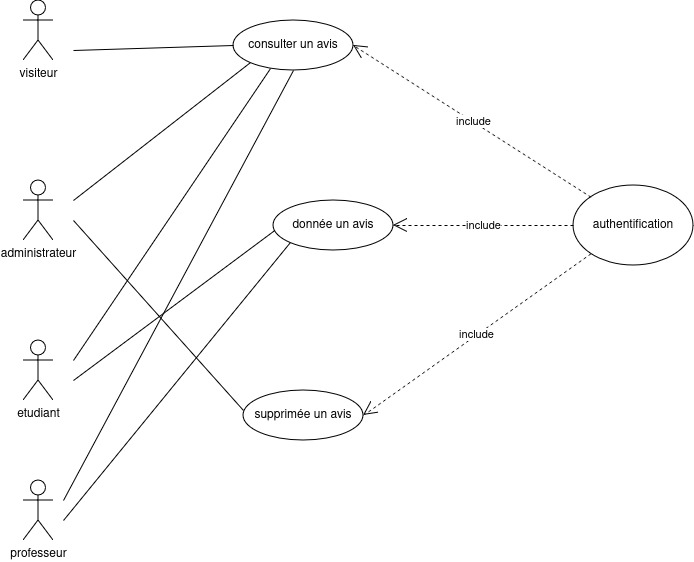
\includegraphics[width=0.7\linewidth]{pages/image/asma-usecase-gestion_des_avis.jpg}
    \caption{ diagramme de cas d'utilisation pour la gestion d'avis}
    \label{fig:enter-label}
\end{figure}
\newpage
\section{Déscription textuelle }

\begin{table*}[h]
    \begin{center} 
    \begin{tabular}{|p{4cm}|p{9cm}|}  \hline 
       Cas d'utilisation& Gestion des avis \\ \hline
       Acteur& Etudiant,Administrateur , visiteur ,professeur\\ \hline
       Précondition&  L'étudiants,l'administrateur ou le professeur doive être authentifiés au plateforme &  \\ \hline
       Post condition& Un avis sera ajouté à la liste des avis.\\ \hline


       
       Scénario nominale& Le systéme affiche la liste des exercies  \\
                        & L'étudiant sélectionne un exercies à le faire \\
                        & L'étudiant termine a faire et va donner un avis sur l'exercies \\
                        & L'admin peut supprimer un avis \\ \hline
          
                       
       Scénario alternatif& Le système renvoie un message d’erreur et signale à l’étudiant de
recommencer en cas d’erreur de synchronisation. \\  \hline
  \end{tabular}
  \end{center}
  \caption{ Déroulement de cas d'utilisation}
\label{tab:bert_res}
\end{table*}

\section{Conception }

La figure  décrit le déroulement du cas d’utilisation « donner un avis » pour le visteur.
\begin{figure}[h!]
    \centering
    \includegraphics[width=0.8\linewidth]{}
    \caption{Diagramme de séquance «Gestion des avis - visiteur»}
    \label{fig:enter-label}
\end{figure}
\\ 

Le diagramme ci-dessous représente le diagramme de séquence du cas d’utilisation « Gestion des avis » pour l'etudiant 
\begin{figure}[h!]
    \centering
    \includegraphics[width=0.8\linewidth]{}
    \caption{Diagramme de séquance «donner un avis - etudiant »}
    \label{fig:enter-label}
\end{figure}
\\


Le diagramme ci-dessous représente le diagramme de séquence du cas d’utilisation « Gestion des avis » pour le professeur 
\begin{figure}[h!]
    \centering
    \includegraphics[width=0.8\linewidth]{}
    \caption{Diagramme de séquance «donner un avis - professeur»}
    \label{fig:enter-label}
\end{figure}
\\


Le diagramme ci-dessous représente le diagramme de séquence du cas d’utilisation « Gestion des avis » pour l'administrateur 
\begin{figure}[h!]
    \centering
    \includegraphics[width=0.8\linewidth]{}
    \caption{Diagramme de séquance «donner un avis - administrateur »}
    \label{fig:enter-label}
\end{figure}
\\


\section{Diagramme de classe condidate}
La figure  représente les différentes classes candidates du ce Sprint.
\begin{figure}[h!]
    \centering
    \includegraphics[width=0.5\linewidth]{}
    \caption{Diagramme de classe "ajouter un avis"}
    \label{fig:enter-label}
\end{figure}

\section{Réalisation}
cette figure représante l'interface des avis données sur les supports de cours pour un visiteur qui n'est pas inscrit au plateforme:

\begin{figure}[h!]
    \centering
    \includegraphics[width=0.5\linewidth]{}
    \caption{Interface utlisateur pour consulter les avis existante}
    \label{fig:enter-label}
\end{figure}
\\

Cette figure représante l'interface des avis données sur les supports de cours pour un étudiant:
\begin{figure}[h!]
    \centering
    \includegraphics[width=0.5\linewidth]{}
    \caption{Interface utilisateur pour un étudiant qui a ajouté un avis}
    \label{fig:enter-label}
\end{figure}


\section{Conclusion:}
En conclusion ,dans cette chapitre nous avons exploré les élements clés de la procedure de la gestion des avis pour notre plateforme
        \clearpage



    %\chapter{Sprint 4 :Gestion des utilisateurs}
        %\label{chap:chaptersix}
        % \input{pages/chapitre/chapitre6}
        \clearpage
\end{document}